\documentclass[a4paper, 11pt]{article}
\usepackage{comment}
\usepackage{fullpage}
\usepackage{amsmath}
\usepackage{amssymb}
\usepackage{mathtools}
\usepackage{fontspec}
\defaultfontfeatures{Ligatures=TeX}
\usepackage{xfrac}
\usepackage{icomma}
\usepackage[section,below]{placeins}
\usepackage[labelfont=bf,font=small,width=0.9\textwidth]{caption}
\usepackage{subcaption}
\usepackage{graphicx}
\usepackage{grffile}
\usepackage{float}
\floatplacement{figure}{htbp}
\floatplacement{table}{htbp}
\usepackage{booktabs}
\usepackage{hyperref}
\usepackage[ngerman]{babel}
\begin{document}
\noindent
%\centerline{\small{\textsc{Technische Universität Dortmund}}} \\
\large{\textbf{3. Übungsblatt zur Vorlesung \hfill WS 2017/2018 \\
Statistische Methoden der Datenanalyse \hfill Prof. W. Rhode}} \\
Annika Burkowitz, Sebastian Bange, Alexander Harnisch \\
\noindent\makebox[\linewidth]{\rule{\textwidth}{0.4pt}}

\section*{Aufgabe 8}
\subsection*{a)}
Die Wahrscheinlichkeit, dass $x$ einen Wert zwischen $\frac{1}{3}$ und $\frac{1}{2}$ annimmt ist gegeben durch
\begin{equation}
    \int_{\frac{1}{3}}^{\frac{1}{2}} f(x) \textup{d}x = \frac{1}{2} - \frac{1}{3} = \frac{1}{6} \,.
\end{equation}

\subsection*{b)}
Die Wahrscheinlichkeit, dass irgendein ein exakter Wert angenommen wird ist 0. Dies ist einerseits klar, weil mit unendlich verschiedenen möglichen Werten sonst nie eine endliche Gesamtwahrscheinlichkeit erreicht werden könnte. Außerdem ist natürlich die integrierte Wahrscheinlichkeitsdichte
\begin{equation}
    \int_{a}^{a} f(x) \textup{d}x = 0 \,.
\end{equation}

\subsection*{c)}
In den folgenden beiden Aufgaben sollen die Zahlen von einem Computer berechnet werden können.
Zur Darstellung soll eine Mantisse mit 23 Binärstellen angenommen werden.
Damit möglichst viele Zahlen zwischen 0 und 1 dargestellt werden können und die Zahlen 0 und 1 ebenfalls in der Menge enthalten sind, wird folgende Darstellung gewählt:
\begin{center}
    \begin{tabular}{c|c}
        Binärdarstellung & Dezimaldarstellung \\
        \toprule
        00000000000000000000000 & 0 \\
        00000000000000000000001 & $\frac{1}{2^{23} - 1}$ \\
        00000000000000000000010 & $2\cdot\frac{1}{2^{23} - 1}$ \\
        \multicolumn{2}{c}{\vdots} \\
        11111111111111111111111 & 1 \\
    \end{tabular}
\end{center}
Dadurch hat jede darstellbare Zahl die Wahrscheinlichkeit $p = 2^{-23}$ aufzutreten.

Um zu testen, ob die Zahl $\frac{1}{2}$ darstellbar ist, wird berechnet, ob $\frac{1}{2}$ ein ganzzahliges Vielfaches von $\frac{1}{2^{23} - 1}$ ist:
\begin{align}
    x \frac{1}{2^{23} - 1} &\overset{!}{=} \frac{1}{2} \\
    \Leftrightarrow x &= \frac{2^{23} - 1}{2} \\
    &= 4194303.5 \not\in \mathbb{N}.
\end{align}
Damit ist die Zahl $\frac{1}{2}$ nicht exakt darstellbar und die Wahrscheinlichkeit sie zu berechnen ist Null.

\subsection*{d)}
Um zu testen, ob die Zahl $\frac{2}{3}$ darstellbar ist, wird berechnet, ob $\frac{2}{3}$ ein ganzzahliges Vielfaches von $\frac{1}{2^{23} - 1}$ ist:
\begin{align}
    x \frac{1}{2^{23} - 1} &\overset{!}{=} \frac{2}{3} \\
    \Leftrightarrow x &= \frac{2(2^{23} - 1)}{3} \\
    &\approx 5592404.66667 \not\in \mathbb{N}.
\end{align}
Damit ist die Zahl $\frac{2}{3}$ nicht exakt darstellbar und die Wahrscheinlichkeit sie zu berechnen ist Null.

\section*{Aufgabe 9}
\subsection*{a)}
Gegeben ist der Linear-kongruenten Zufallszahlengenerator
\begin{equation}
    x_n = (ax_{n-1} + b)\ \textup{mod}\ m
    \label{eqn:linkon}
\end{equation}
mit $b = 3$ und $m = 1024$. Damit ist sofort klar, dass die maximale auftretende Periodenlänge nicht größer als $m = 1024$ sein kann. Wir bestimmen die Periodenlänge für alle $a$ von 0 bis 1024. Das Ergebnis ist in Abbildung~\ref{fig:9a_full} dargestellt. Zusätzlich ist in Abilldung~\ref{fig:9a_zoom} der Bereich für $a$ von 0 bis 32 höher aufgelöst dargestellt. Für die erzeugten Abbildungen wurde der Startwert $x_0 = 1$ verwendet, das Ergebnis ist unseren Tests nach jedoch unabhängig vom Startwert. Die maximale Periodenlänge ist wie erwartet $2^{10} = 1024$.
\begin{figure}
    \centering
    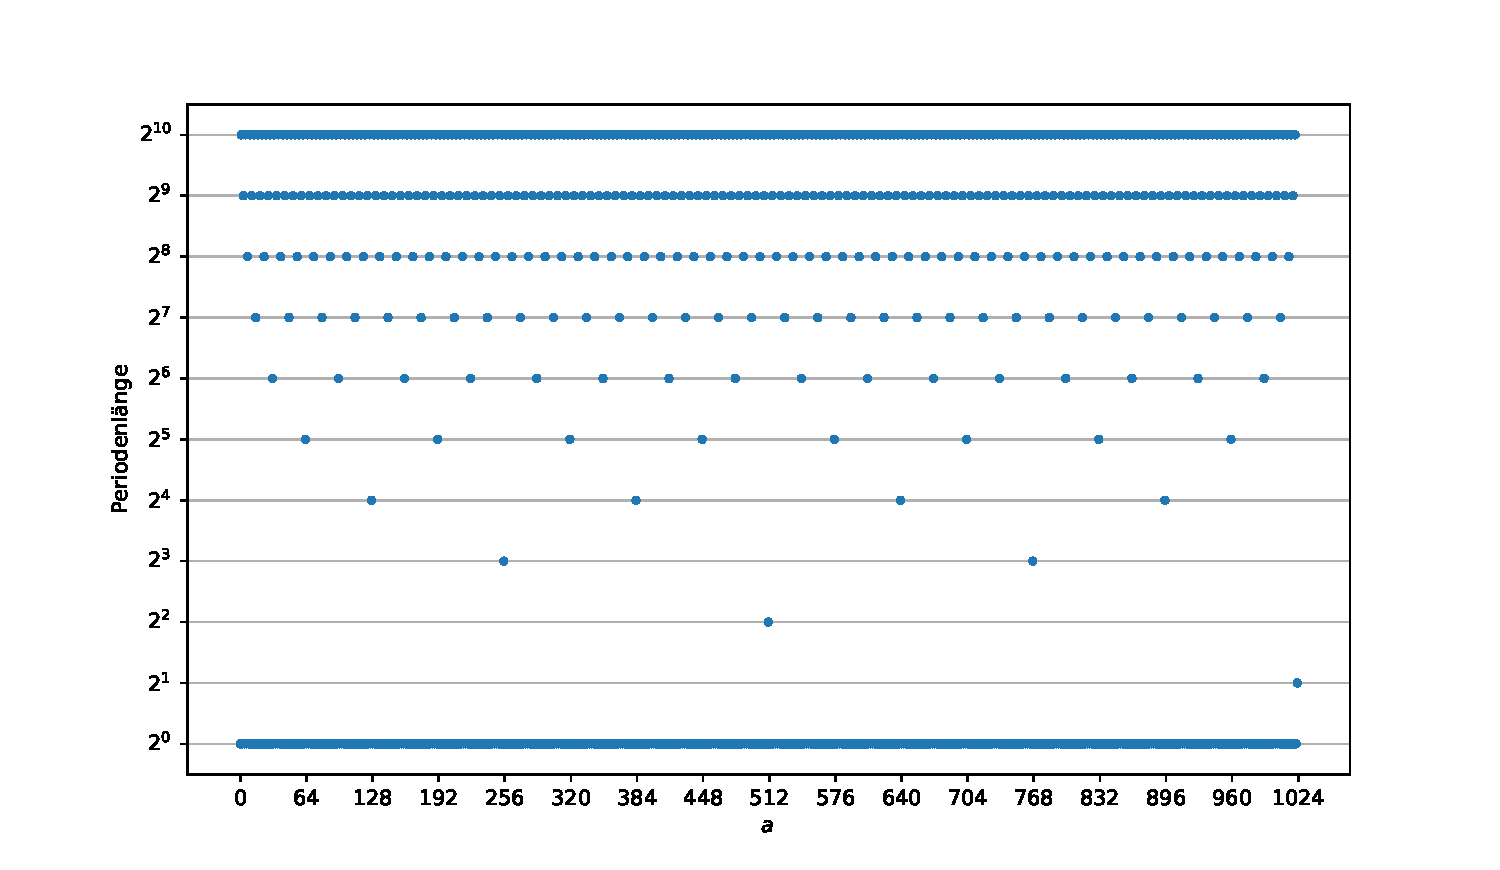
\includegraphics[width=\textwidth]{../A09/A9a_full.pdf}
    \caption{Periodenlänge für alle $a$ von 0 bis 1024.}
    \label{fig:9a_full}
\end{figure}
\begin{figure}
    \centering
    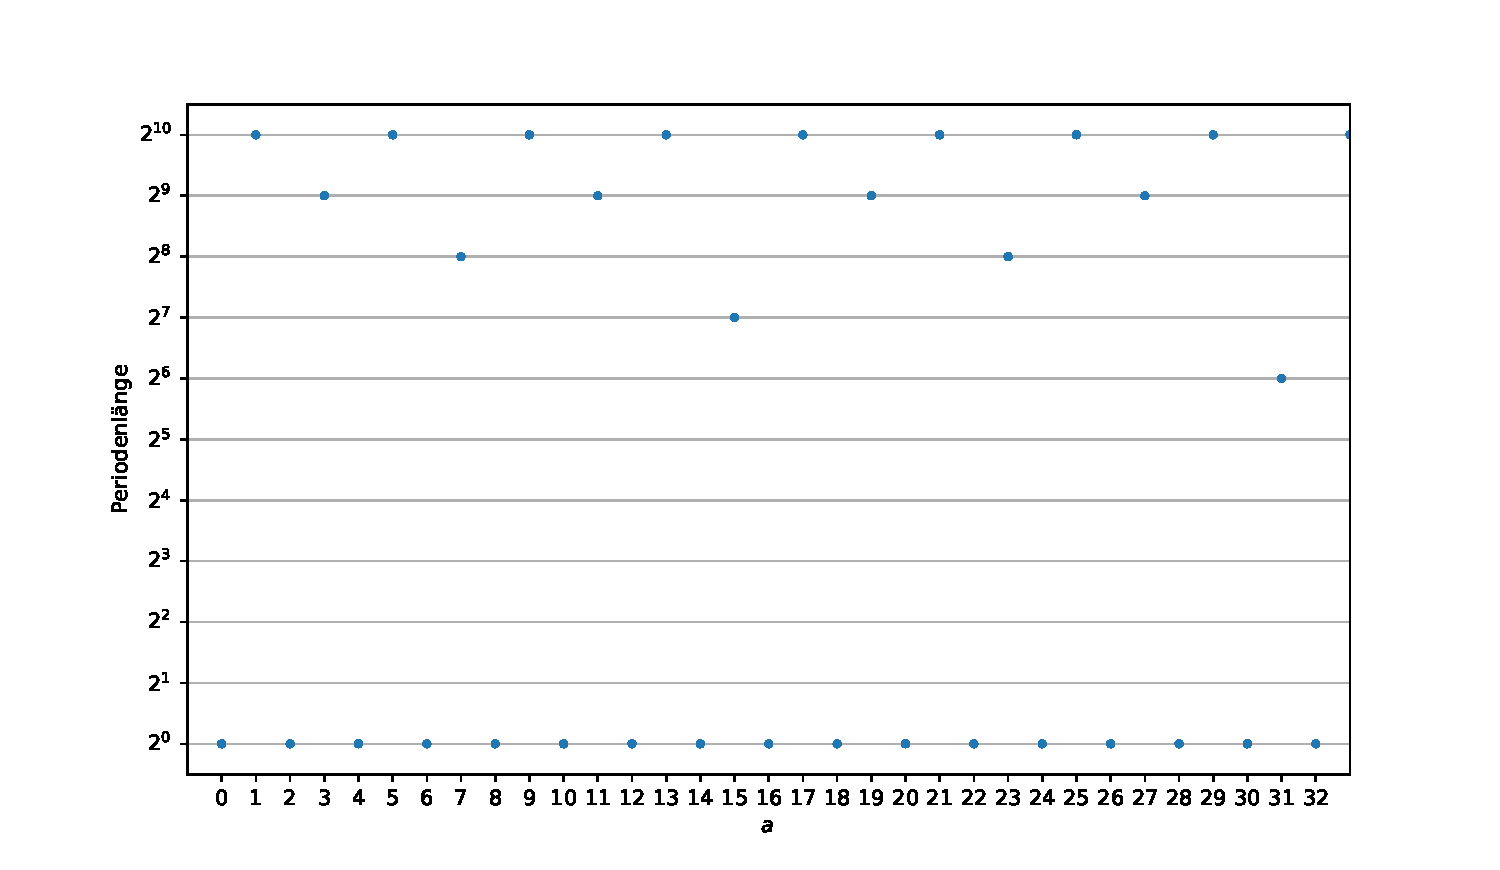
\includegraphics[width=\textwidth]{../A09/A9a_zoom.pdf}
    \caption{Periodenlänge für alle $a$ von 0 bis 32.}
    \label{fig:9a_zoom}
\end{figure}

Das Verhalten lässt sich sehr gut durch die Regeln für gute linear-kongruente Generatoren~\cite[S.~7]{skript} erklären: Die Regeln 1 und 2 sind erfüllt. Die Regel 3 ist für alle ungeraden Zahlen erfüllt, da die Primfaktorzerlegung von $m$ durch $2^{10}$ gegeben ist. Wie gut zu erkennen ist, ist die Periodenlänge für alle geraden $a$ minimal eins, was die Regel bestätigt. Für alle $a$, für die gilt, dass $a-1$ außerdem durch 4 teilbar ist (Regel 4) ist die Periodenlänge maximal. Leider haben wir gerade keine Zeit mehr uns länger Gedanken darüber zu machen, welchen Regeln die übrigen Werte folgen, aber offenbar bildet sich bei jedem $a+1 = 2^{n}$ eine neue Ebene mit der Periodenlänge $2^{11 - n}$.
\FloatBarrier

\subsection*{c)}
Das geforderte Histogramm ist durch Abbildung~\ref{fig:a9c} gegeben. Das Ergebnis wurde für viele verschiedene Startwerte berechnet und scheint unabhängig von diesem zu sein. Es entspricht nicht den Anforderungen an einen guten Zufallszahlengenerator, da offenbar keine echte Gleichverteilung vorliegt, sondern manche Zahlen signifikant wahrscheinlicher sind als andere.
\begin{figure}
    \centering
    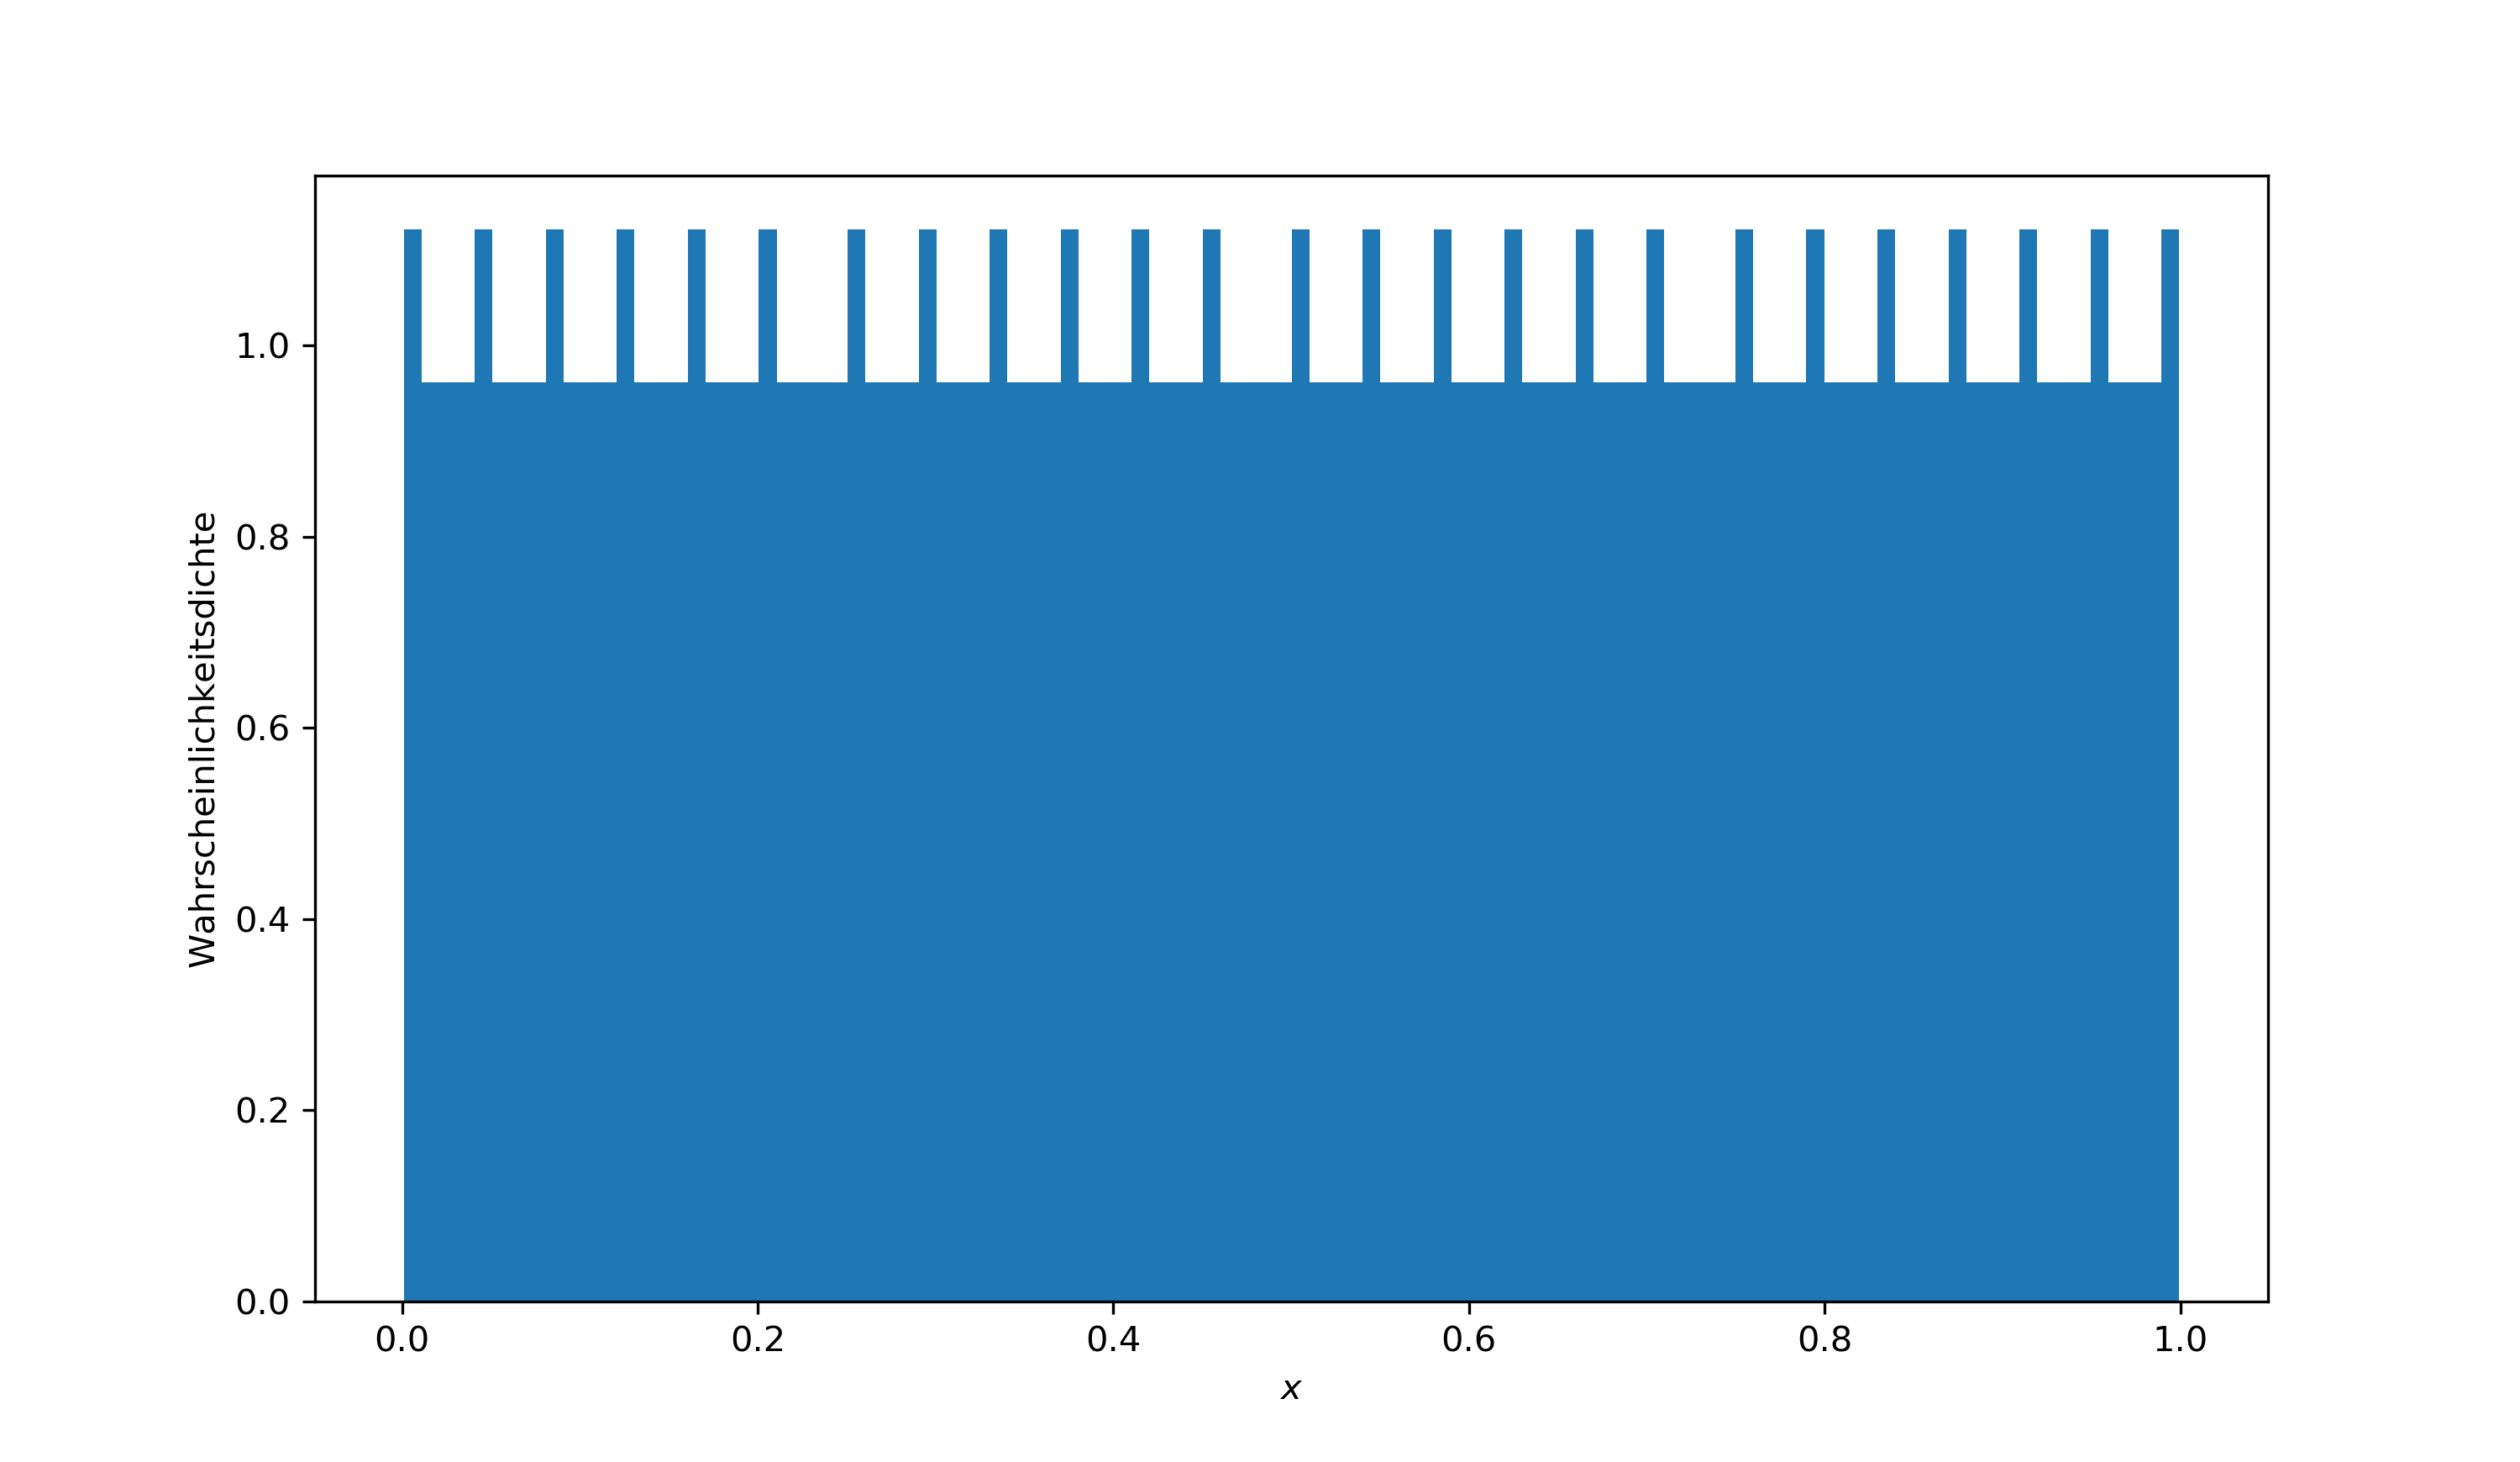
\includegraphics[width=\textwidth]{../A09/A9c.png}
    \caption{Histogramm für 10000 nach~\ref{eqn:linkon} erzeugte Zufallszahlen. }
    \label{fig:a9c}
\end{figure}
\FloatBarrier

\subsection*{d)}
Die geforderten Streudiagramme sind durch die Abbildungen~\ref{fig:a9d_2d} und~\ref{fig:a9d_3d} gegeben. Es ist klar zu erkennen, dass die Zahlen von einem schlechten Zufallszahlengenerator generiert wurden, da sich Ebenen bilden. Es besteht also eine vorhersagbare Korrelation zwischen aufeinanderfolgenden Zufallszahlen.
\begin{figure}
    \centering
    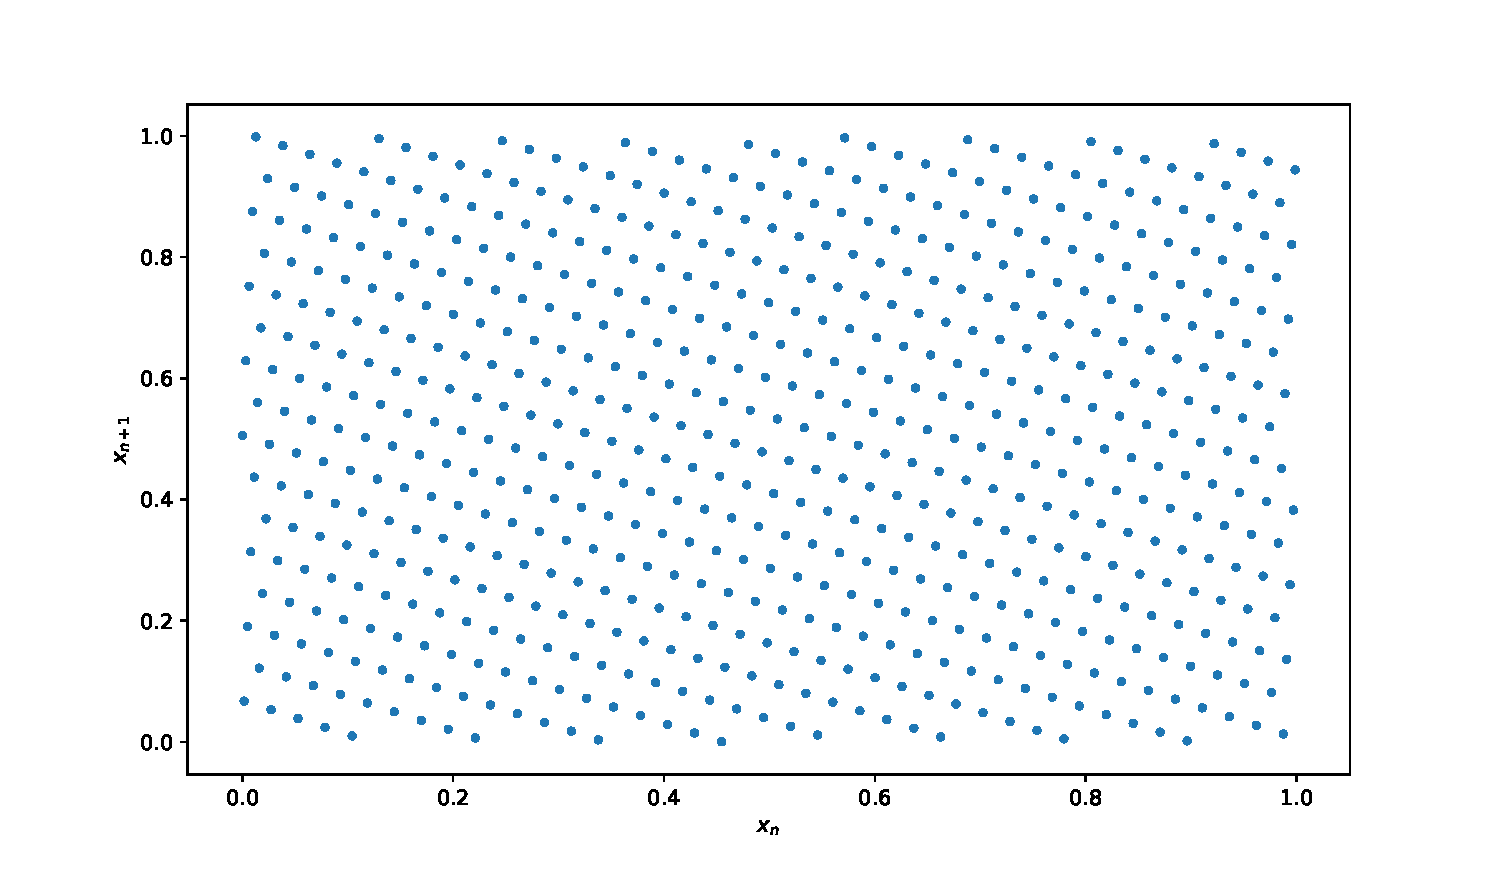
\includegraphics[width=\textwidth]{../A09/A9d_2D.pdf}
    \caption{Zweidimensionales Streudiagramm für den Linear-kongruenten Zufallszahlengenerator.}
    \label{fig:a9d_2d}
\end{figure}
\begin{figure}
    \centering
    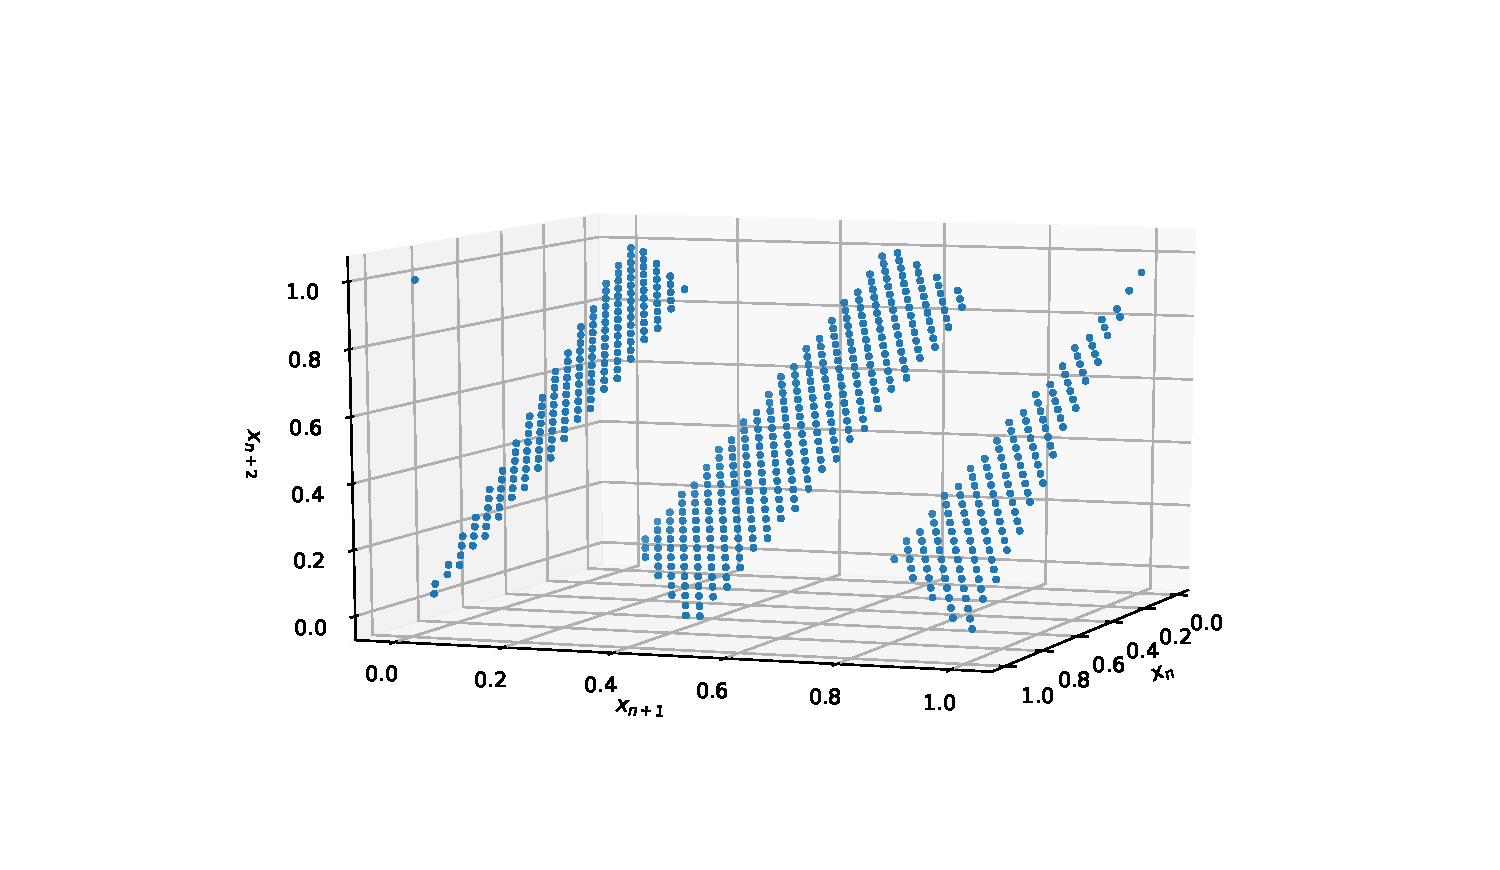
\includegraphics[width=\textwidth]{../A09/A9d_3D.pdf}
    \caption{Dreidimensionales Streudiagramm für den Linear-kongruenten Zufallszahlengenerator.}
    \label{fig:a9d_3d}
\end{figure}
\FloatBarrier

\subsection*{e)}
Die geforderten Streudiagramme sind durch die Abbildungen~\ref{fig:a9e_2d} und~\ref{fig:a9e_3d} gegeben. Es ist klar zu erkennen, dass die Zahlen von einem guten Zufallszahlengenerator generiert wurden, da sich keine erkennbaren Muster bilden. Es besteht also keine vorhersagbare Korrelation zwischen aufeinanderfolgenden Zufallszahlen.
\begin{figure}
    \centering
    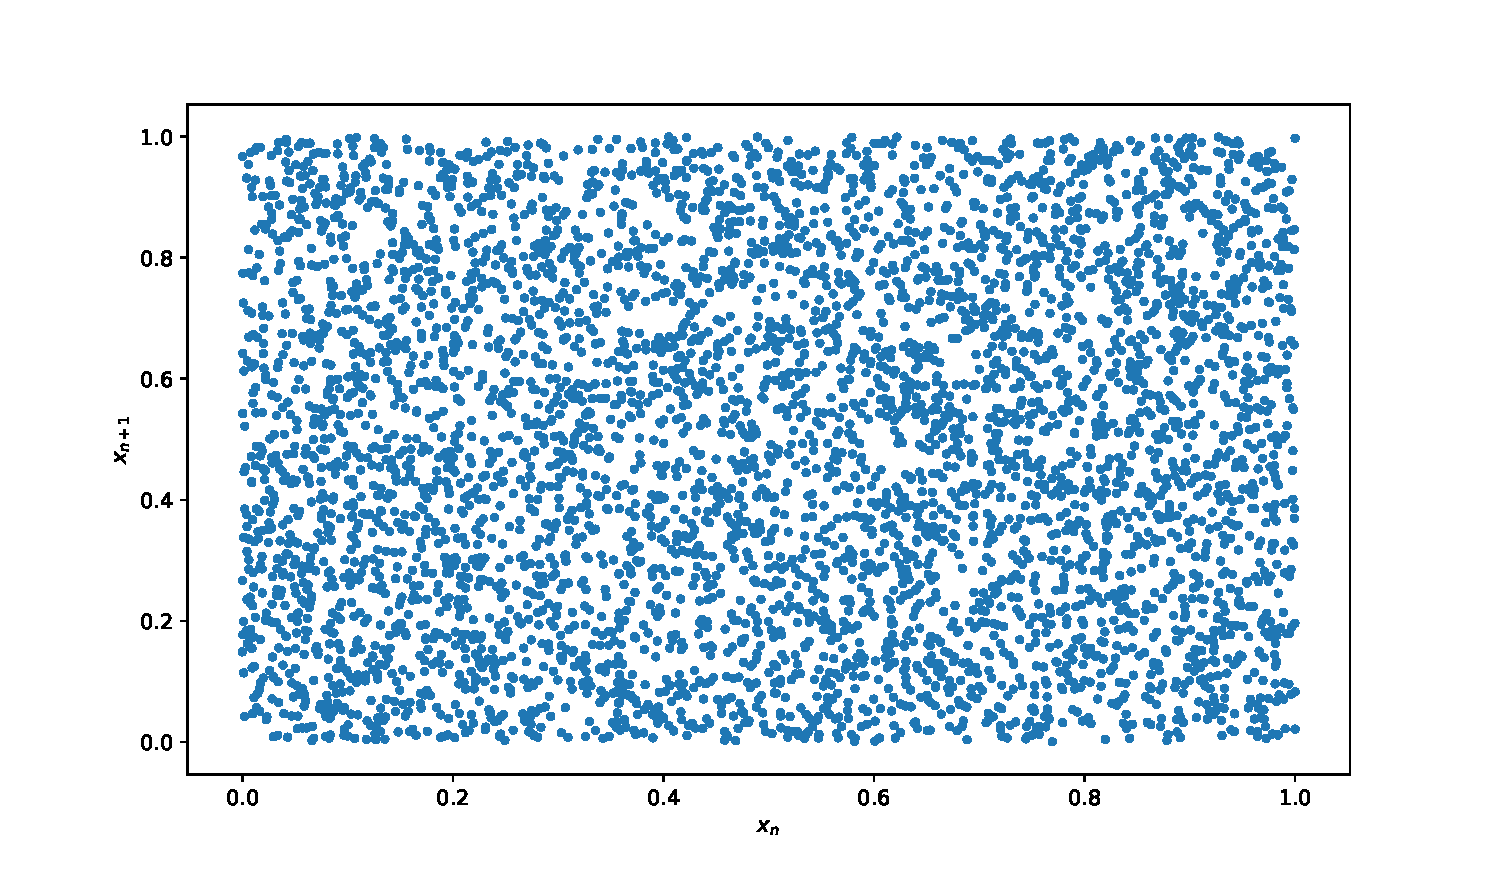
\includegraphics[width=\textwidth]{../A09/A9e_2D.pdf}
    \caption{Zweidimensionales Streudiagramm für den \textsc{Numpy} Zufallszahlengenerator.}
    \label{fig:a9e_2d}
\end{figure}
\begin{figure}
    \centering
    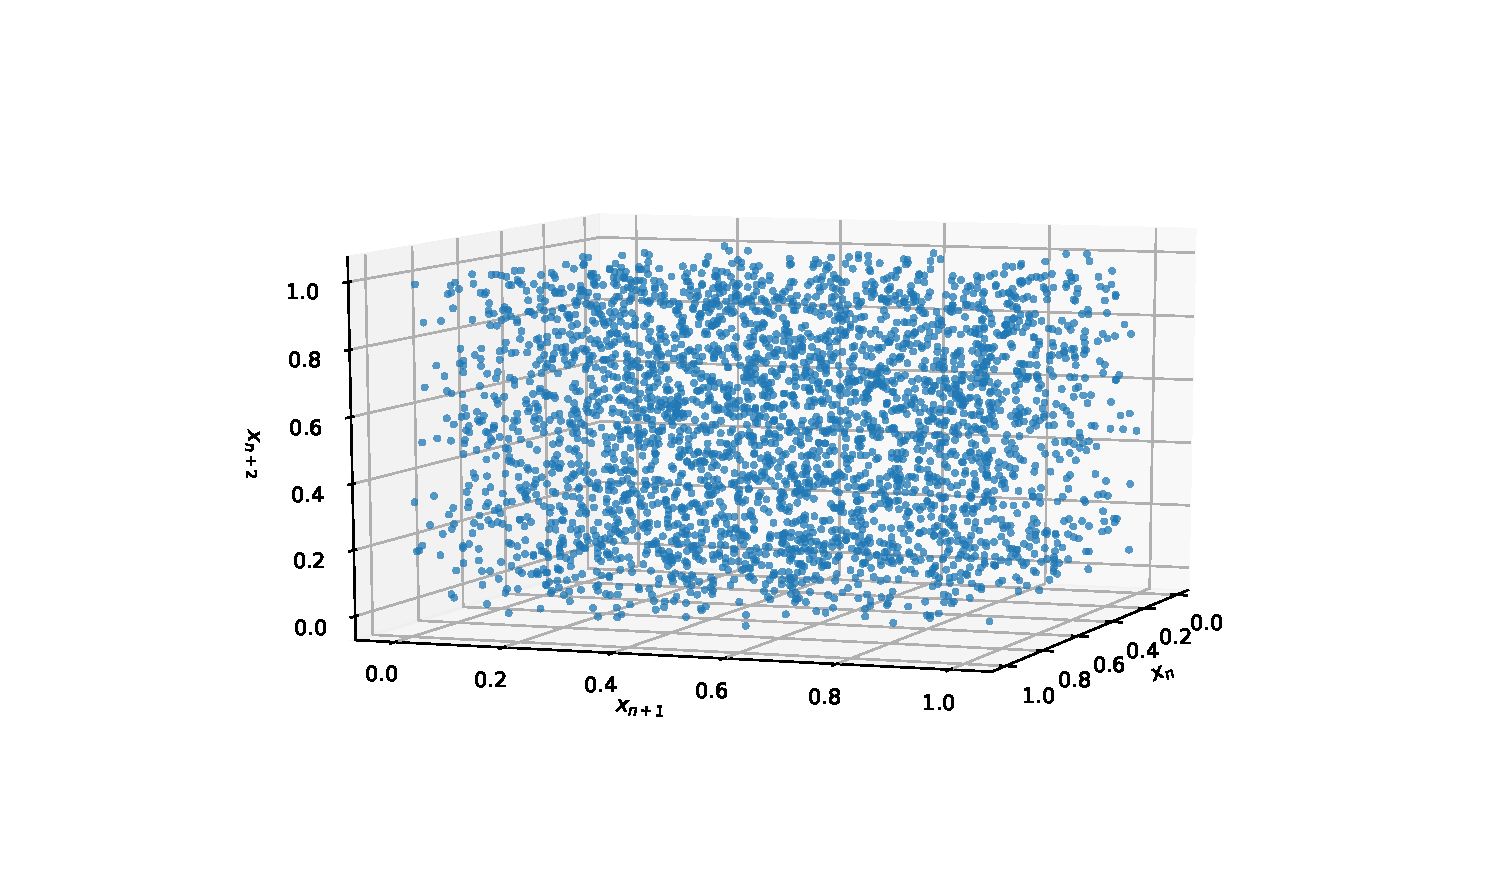
\includegraphics[width=\textwidth]{../A09/A9e_3D.pdf}
    \caption{Dreidimensionales Streudiagramm für den \textsc{Numpy} Zufallszahlengenerator.}
    \label{fig:a9e_3d}
\end{figure}
\FloatBarrier

\subsection*{f)}
Die vom Zufallszahlengenerator generierten Zahlen bestehen für alle Startwerte, die ungerade Vielfache von 8 sind, zu 0,16\,\% aus dem Wert $\frac{1}{2}$. Für alle anderen Startwerte wird nie der Wert $\frac{1}{2}$ generiert. 

\section*{Aufgabe 10}
Für die Gleichverteilung nutzen wir in der gesamten Aufgabe den Zufallszahlengenerator von \textsc{Numpy}. Nach Teilaufgabe \textbf{a)} verwenden wir diesen auch für die Generation von gleichverteilten Zufallszahlen mit anderen Grenzen als 0 und 1, obwohl dies streng genommen nach Aufgabenstellung nicht erlaubt ist, es macht aber keinen Unterschied und ist so vermutlich etwas schneller in der Ausführung. Es könnte auch überall im Code einfach die \textsc{Numpy} Funktion durch unsere selbst implementierte Variante ersetzt werden.

Wir gehen davon aus, dass in den Teilaufgaben \textbf{b)} bis \textbf{d)} mit $f$ gewünshte Dichtefunktionen, und keine kommulierten Wahrscheinlichkeitsfunktionen gemeint sind.

\subsection*{a)}
Gleichverteilte Zahlen zwischen $x_\textup{min}$ und $x_\textup{max}$ lassen sich einfach generieren, indem die zwischen 0 und 1 gleichverteilten Zahlen $z$ nach
\begin{equation} 
    x = (x_\textup{max} - x_\textup{min})z + x_\textup{min}
    \label{eqn:unitrans}
\end{equation}
transformiert werden. Ein Histogramm einer auf diese Weise mit den Grenzen $x_\textup{min} = 2$ und $x_\textup{max} = 5$ generierten Verteilung ist zur Verifikation in Abbildung~\ref{fig:a10a} dargestellt.
\begin{figure}
    \centering
    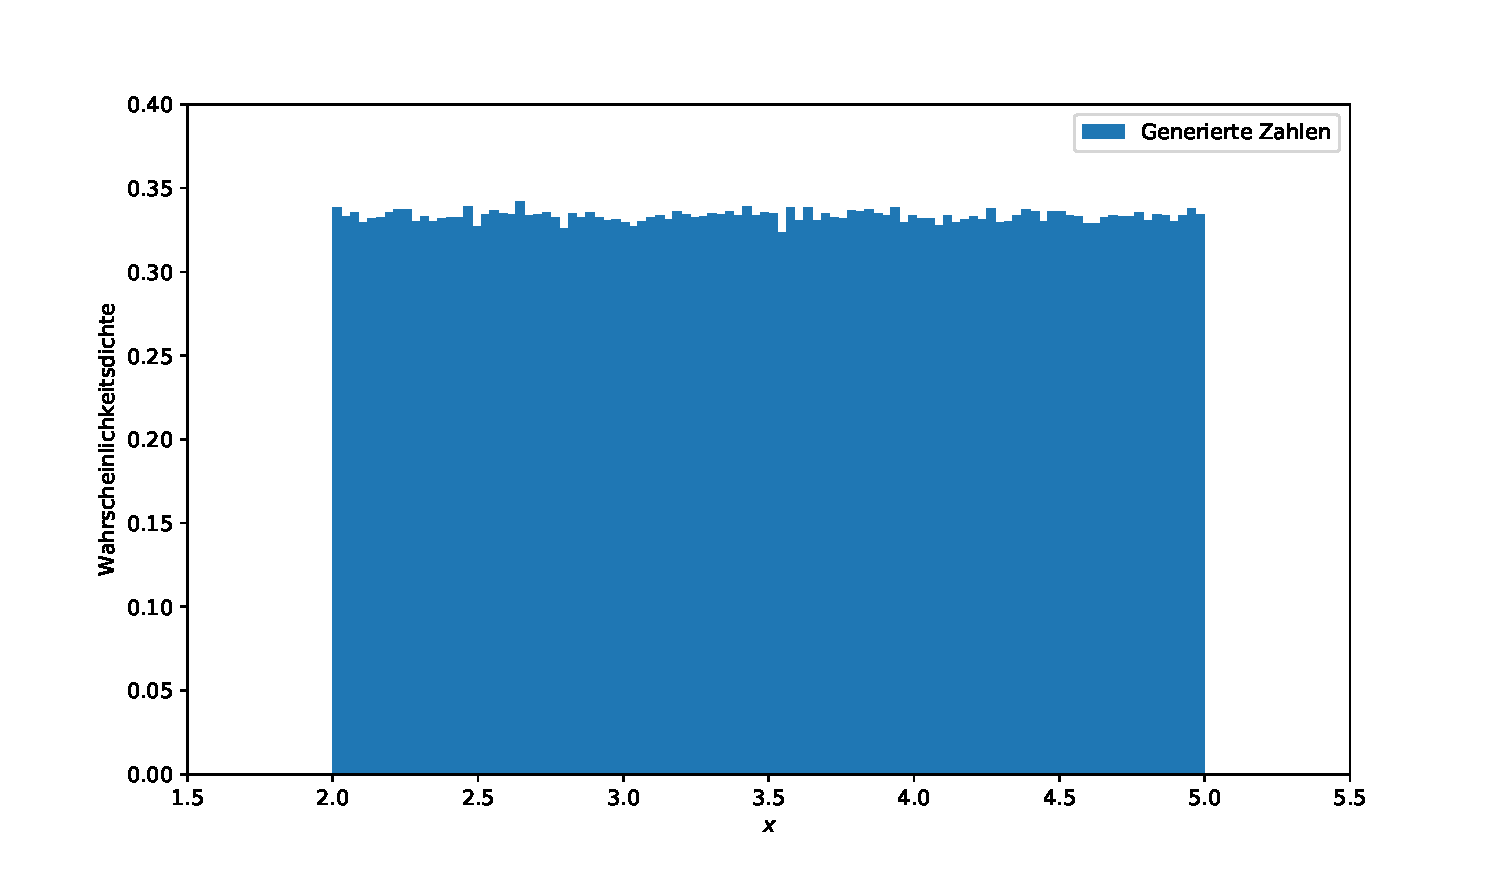
\includegraphics[width=\textwidth]{../A10/A10a.pdf}
    \caption{Histogramm der transformierten Gleichverteilung mit den Grenzen $x_\textup{min} = 2$ und $x_\textup{max} = 5$.}
    \label{fig:a10a}
\end{figure}
\FloatBarrier


\subsection*{b)}
Die gewünschte Dichtefunktion 
\begin{equation}
    f(t) = N \exp\left(-\frac{t}{\tau}\right),\quad t \in [0, \infty)
\end{equation}
lässt sich integrieren. Daher kann zur Erzeugung dieser Verteilung die Transformationsmethode verwendet werden. Für die Verteilungsfunktion ergibt sich\begin{equation}
    F(t) = \int_{0}^{t} N \exp\left(-\frac{x}{\tau}\right) \textup{d}x = 1 - \frac{\exp\left(-\frac{t}{\tau}\right)}{\tau}\,,
\end{equation}
mit der Normierungskonstante $N = \tau^{-1}$. Diese kann nun invertiert werden:
\begin{align}
    z = F(x) &= 1 - \frac{\exp\left(-\frac{t}{\tau}\right)}{\tau} \\
    \Leftrightarrow (1 - z)\tau &= \exp\left(\frac{x}{\tau}\right) \\
    \Rightarrow x &= -\tau \log\left((1-z)\tau\right) \,, \quad z \in \left[1 - \frac{1}{\tau}, 1\right]\,.
\end{align}
Wenn $z$ gleichverteilte Zufallszahlen mit den angegebenen Grenzen sind, dann sind die so transformierten $x$ mit der gewünschten Dichte $f$ verteilt. $z$ kann hier natürlich wieder gemäß \eqref{eqn:unitrans} erzeugt werden, diese Transformation ließe sich auch direkt hier einsetzen. Zur Verifikation erstellen wir auf diese Weise ein Histogramm mit $\tau = 1$, dieses ist in Abbildung~\ref{fig:a10b} dargestellt. 
\begin{figure}
    \centering
    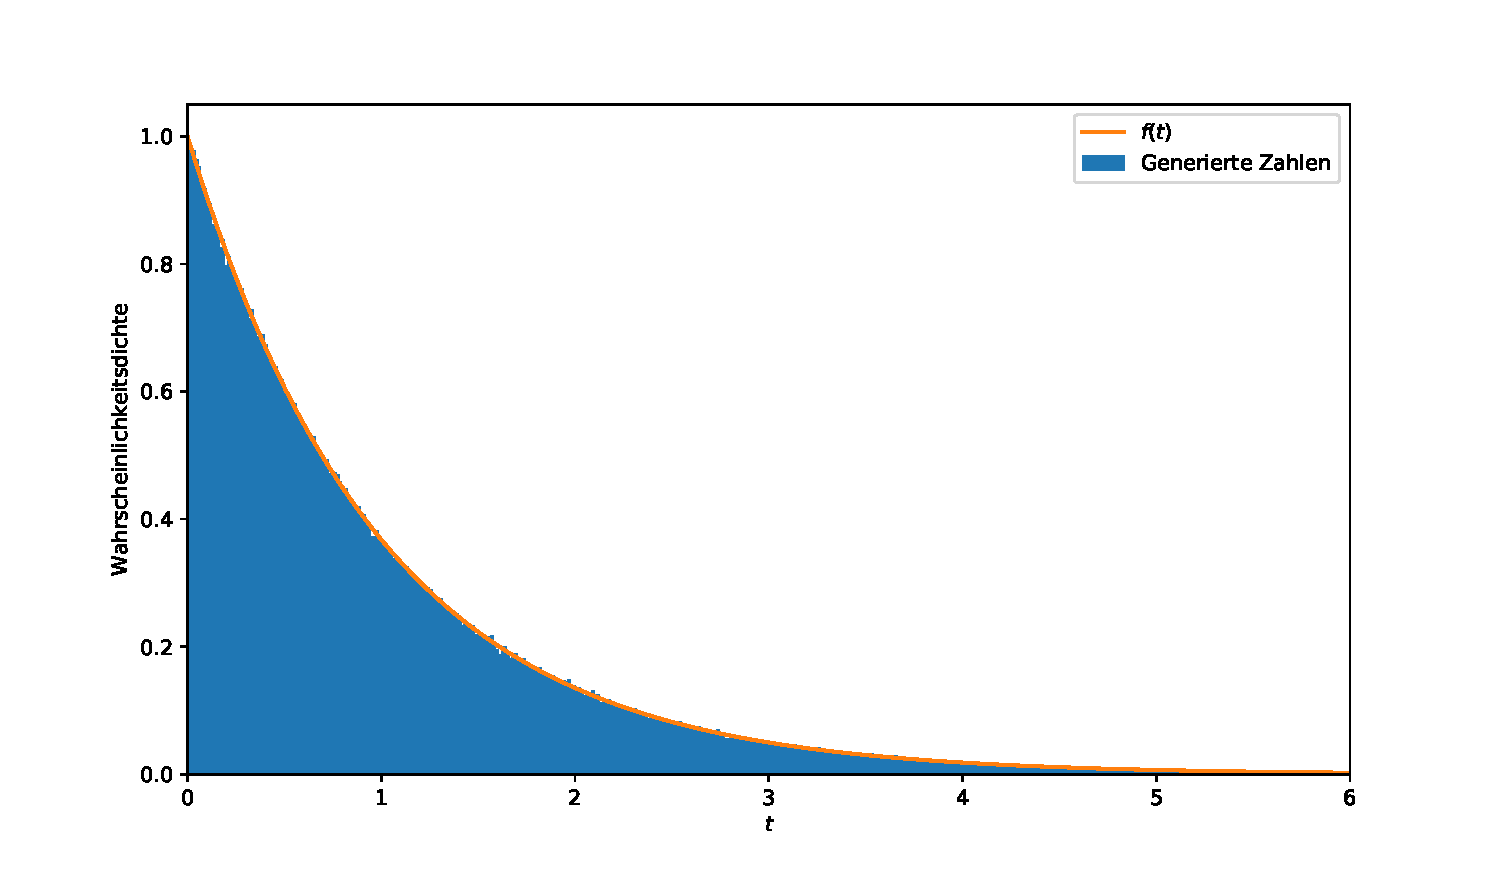
\includegraphics[width=\textwidth]{../A10/A10b.pdf}
    \caption{Histogramm der generierten Verteilung aus Aufgabe 10b).}
    \label{fig:a10b}
\end{figure}
\FloatBarrier

\subsection*{c)}
Die gewünschte Dichtefunktion 
\begin{equation}
    f(x) = Nx^{-n},\quad x \in [x_{\textup{min}}, x_\textup{max}]
\end{equation}
mit $n\geq2$ lässt sich integrieren. Daher kann zur Erzeugung dieser Verteilung erneut die Transformationsmethode verwendet werden. Für die Verteilungsfunktion ergibt sich\begin{equation}
    F(x) = \int_{x_\textup{min}}^{x} f(x') \textup{d}x' = \frac{N}{1 - n}\left(x^{1 - n} - x_\textup{min}^{1 -n}\right), \quad x \in [x_\textup{min}, x_\textup{max}]
\end{equation}
mit der Normierungskonstante 
\begin{equation}
    N = \frac{1 - n}{x_\textup{max}^{1- n} - x_\textup{min}^{1 - n}}\,.
\end{equation}
Diese kann nun invertiert werden:
\begin{gather}
    z = F(x) \\
    \Rightarrow x = \left(z(x_\textup{max}^{1-n} - x_\textup{min}^{1-n}) + x_\textup{min}^{1-n}\right)^{\frac{1}{1-n}}, \quad z \in [0,  1]\,.
\end{gather}
Wenn $z$ gleichverteilte Zufallszahlen zwischen 0 und 1 sind, dann sind die so transformierten $x$ mit der gewünschten Dichte $f$ verteilt. Es ist zu erkennen, dass sich hier von selbst die Transformation \eqref{eqn:unitrans} ergeben hat. Zur Verifikation erstellen wir auf diese Weise ein Histogramm mit $n = 2$ und den Grenzen $x_\textup{min} = 1$ und $x_\textup{max} = 5$, dieses ist in Abbildung~\ref{fig:a10c} dargestellt. 
\begin{figure}
    \centering
    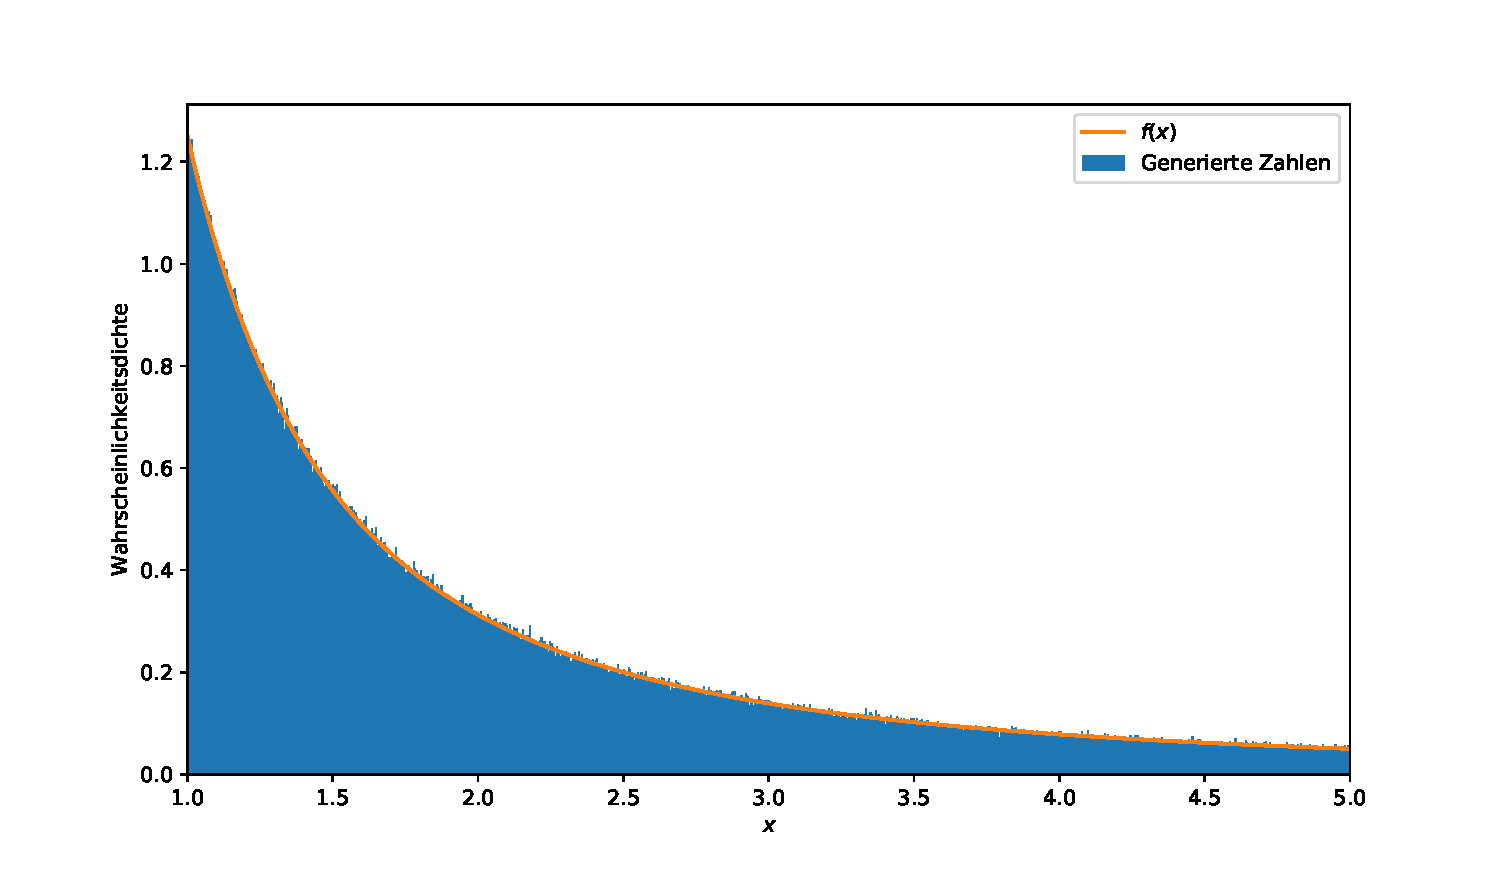
\includegraphics[width=\textwidth]{../A10/A10c.pdf}
    \caption{Histogramm der generierten Verteilung aus Aufgabe 10c).}
    \label{fig:a10c}
\end{figure}
\FloatBarrier

\subsection*{d)}
Die Wahrscheinlichkeitsdichte der \textsc{Cauchy}-Verteilung
\begin{equation}
    f(x) = \frac{1}{\pi}\frac{1}{1 + x^2}\,, \quad x \in (-\infty, \infty)
\end{equation}
ist bereits normiert und lässt sich integrieren. Daher verwenden wir wieder die Transformationsmethode. Die Verteilungsfunktion lautet
\begin{equation}
    F(x) = \frac{1}{\pi} \int_{-\infty}^{\infty} f(x') \textup{d}x' = \frac{\arctan{x}}{\pi} + \frac{1}{2}\,.
\end{equation}
Invertieren der Verteilungsfunktion ergibt
\begin{gather}
    F(x) = z \\
    \Rightarrow x = -\cot(\pi z)\,, \quad z \in [0, 1]
\end{gather}
Wenn $z$ gleichverteilte Zufallszahlen zwischen 0 und 1 sind, dann sind die so transformierten $x$ \textsc{Cauchy}-verteilt. Zur Verifikation erstellen wir auf diese Weise ein Histogramm, dieses ist in Abbildung~\ref{fig:a10d} dargestellt. 
\begin{figure}
    \centering
    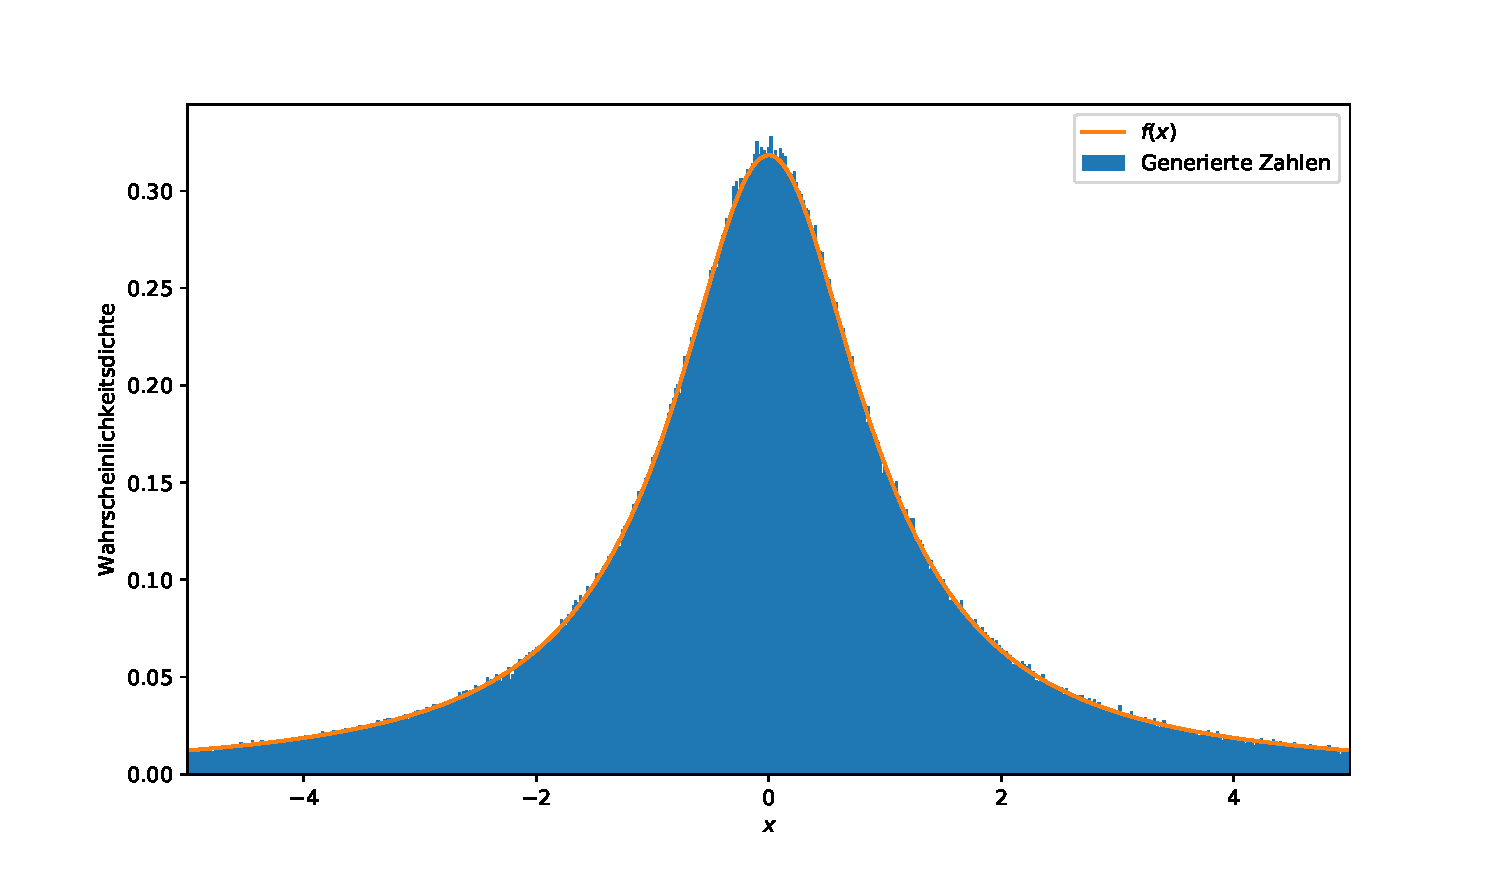
\includegraphics[width=\textwidth]{../A10/A10d.pdf}
    \caption{Histogramm der generierten Verteilung aus Aufgabe 10d).}
    \label{fig:a10d}
\end{figure}
\FloatBarrier

\subsection*{e)}
Es gibt verschiedene Möglichkeiten Zufallszahlen nach einer empirischen Verteilung zu erzeugen. Am einfachsten wäre es vermutlich, die Rückweisungsmethode zu verwenden. Diese ist allerdings sehr ineffizient und deswegen langsam. Stattdessen berechnen wir aus den gegebenen Histogrammdaten die kommulierten Wahrscheinlichkeiten und interpolieren daraus die Inverse der Verteilungsfunktion. Anwenden dieser auf gleichverteilte Zufallszahlen liefert Zahlen, die nach der empirischen Verteilung verteilt sein sollten. Zur Verfikation erstellen wir erneut ein Histogramm, dieses ist zusammen mit dem ursprünglich gegebenen Histogramm in Abbildung~\ref{fig:a10e} dargestellt.

Unsere Vorgehensweise scheint relativ gut zu funktionieren, allerdings scheint es so, als wären die Wahrscheinlichkeiten bei aufsteigenden Flanken etwas zu hoch, und bei abfallenden etwas zu niedrig. Dies kommt vermutlich dadurch zu Stande, dass die Stützstellen in den Mitten der Bins liegen und so beim Bilden der kommulierten Wahrscheinlichkeiten bei steigenden Flanken immer bereits ein halber Bin zu viel, und bei fallenden ein halber zu wenig in den Stützpunkt einfließt. Außerdem ist zu sagen, dass nur sehr wenig Daten gegeben sind, und die zu Grunde liegende Verteilung daher sowieso nur sehr ungenau bekannt ist.
\begin{figure}
    \centering
    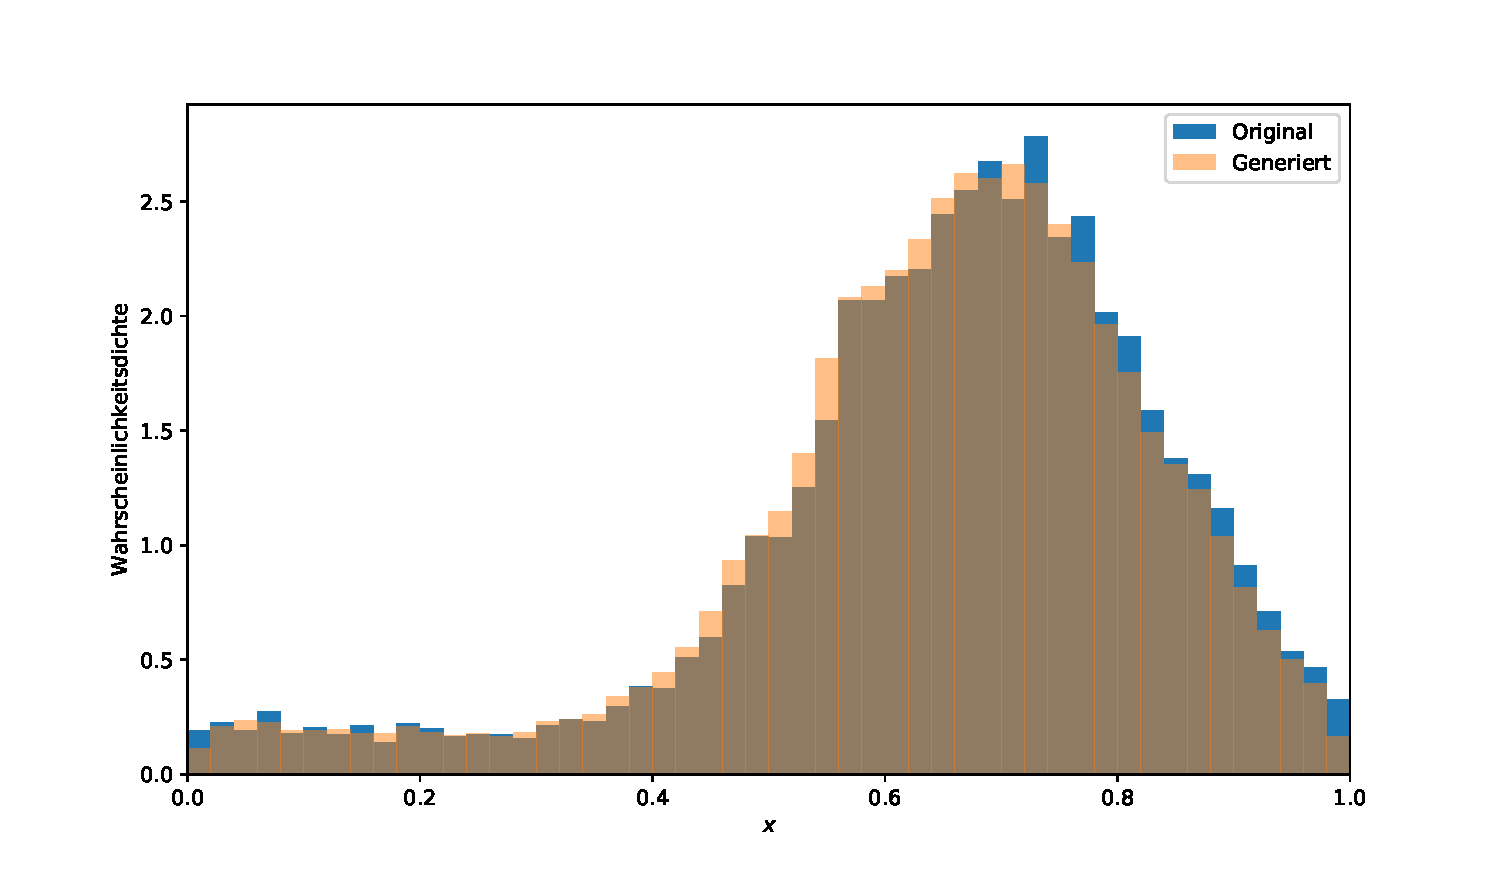
\includegraphics[width=\textwidth]{../A10/A10e.pdf}
    \caption{Darstellung des mittels interpolierter Verteilungsfunktion generierten Histogramms zusammen mit dem ursprünglichen Histogramm aus Aufgabe 10e)}
    \label{fig:a10e}
\end{figure}
\FloatBarrier


\begin{thebibliography}{9}
    \bibitem{skript}
    Wolfgang Rhode
    \textit{Generation von Zufallszahlen}
    \url{https://moodle.tu-dortmund.de/pluginfile.php/618120/mod_resource/content/1/Generation\%20Zufallszahlen.pdf}
\end{thebibliography}
\end{document}
